\documentclass[a4paper]{exam}
\usepackage{amsmath,amssymb,amsthm}
\usepackage{listings}
\usepackage{xcolor} % Optional, for color
\usepackage{geometry}
\usepackage{graphicx}
\usepackage{hyperref}
\usepackage{float}
\usepackage{multirow}
\usepackage{array}
\usepackage{titling} % Required for the subtitle command
\usepackage{pythonhighlight}
\usepackage{graphicx}
\usepackage{tikz}
\usepackage{caption}

\definecolor{codegreen}{rgb}{0,0.6,0}
\definecolor{codegray}{rgb}{0.5,0.5,0.5}
\definecolor{codepurple}{rgb}{0.58,0,0.82}
\definecolor{backcolour}{rgb}{0.95,0.95,0.92}

\lstdefinestyle{mystyle}{
    backgroundcolor=\color{backcolour},   
    commentstyle=\color{codegreen},
    keywordstyle=\color{magenta},
    numberstyle=\tiny\color{codegray}, % Adjust font size and color
    stringstyle=\color{codepurple},
    basicstyle=\ttfamily\footnotesize,
    breakatwhitespace=false,         
    breaklines=true,                 
    captionpos=b,                    
    keepspaces=true,                 
    numbers=left, % Line numbers on the left
    numbersep=5pt,                  
    showspaces=false,                
    showstringspaces=false,
    showtabs=false,                  
    tabsize=2,
    firstnumber=1 % Start line numbers at 1
}


\lstset{style=mystyle}


\setlength{\droptitle}{-1.5in} % Adjust this value to decrease the spacing above the title

\title{EE-424L Data Communication and Networking\\
ASSIGNMENT NO.1}

\author{Syed Ahad Ali\\
sa07753\\
L2}


\date{\today}

\printanswers % This command enables the display of answers


\begin{document}

    \maketitle
    % \vspace{-3cm} % Adjust this value to decrease the spacing below the title

    \begin{center}
        \textbf{Fall 2024}\\
        \textbf{Habib University}\\
        \textbf{Dhanani School of Science \& Engineering}\\
        \textbf{TOTAL MARKS:100}\\
        \textbf{OBTAINED MARKS:}
    \end{center}

    % \vspace{1cm} % Adjust this value to decrease the spacing below the title

    \section*{Purpose}
    The purpose of this assignment is to help you apply the concepts of data communication modes, network models, protocol layering, and network types.

    \section*{Instructions}
    \begin{enumerate}
        \item This assignment should be done individually.
        \item All questions should be answered in black ink only. (Extra sheets can be used)
        \item Scan your answer sheet and upload it on LMS before the due date.
    \end{enumerate}

    \section*{Grading Criteria}
    \begin{enumerate}
        \item Your assignments will be checked by the instructor/TA.
        \item You may be asked to give a viva where you will be judged on whether you understood the questions yourself. If you are unable to correctly answer the question you have attempted, you may lose your marks.
        \item Zero will be given if the assignment is found to be plagiarized.
        \item Untidy work will result in a reduction of your points.
    \end{enumerate}

    \section*{Late Submission Penalty}
    \begin{itemize}
        \item 1-day late submission – 4\% deduction of the maximum allowable marks.
        \item 2-days late submission – 8\% deduction of the maximum allowable marks.
        \item No submission will be accepted after one week of the original deadline.
    \end{itemize}

    \pagebreak

    \section*{CLO Assessments}
    \begin{table}[h]
        \centering
        \begin{tabular}{|p{2cm}| p{10cm}| p{3cm}|} % Adjust the widths as needed
        \hline
        \multicolumn{2}{|c|}{Course Learning Outcomes} & \multicolumn{1}{c|}{CLO Assessed} \\ \hline
        CLO 1 & To compare and classify different data signals, physical transmission medium, topologies, error, and flow control at the data link layer of the computer networks. & \makebox[3cm][c]{\raisebox{0.5\height}{\checkmark}} \\ \hline
        CLO 2 & To orient different functionalities, protocol stacks, and architecture of the Network, Transport, and Application layers of data network models. & \\ \hline
        CLO 3 & To investigate different network functionalities (e.g., security, computing, virtualization, etc.) and relate them with state-of-the-art research scenarios, such as Software Defined Networks (SDN) and the Internet of Things (IoT). & \\ \hline
        \end{tabular}
    \end{table}

    \begin{questions}
        \question[10]{Most data communication in a computer network uses serial transfer as compared to parallel transfer of data which is used in computer peripherals. Can you find out and explain the reason why serial communication is the preferred mode of data transfer in networking devices?}
        \begin{solution}
            There are many reasons for that and few are stated below:
            \begin{parts}
                \item \textbf{Cost:} Serial communication is cheaper than parallel communication. This is because serial communication requires fewer wires and components due to transmitting only one bit at a time and using fewer I/O pins.
                \item \textbf{Distance:} Serial communication can be used over longer distances than parallel communication. This is because serial communication is less susceptible to noise and interference.
                \item \textbf{Simplicity:} Serial communication is simpler to implement than parallel communication. This is because serial communication requires fewer wires and components, making it easier to design and build.
                \item \textbf{Low Production Cost:} Serial communication is cheaper to produce than parallel communication. This is because serial communication requires fewer wires and components, making it less expensive to manufacture.
            \end{parts}

            % References for the solution
            \begin{thebibliography}{9} 
                \bibitem{author1}
                \url{https://www.fullyinstrumented.com/serial-communication/}
                
                \bibitem{author2}
                \url{https://en.wikipedia.org/wiki/Serial_communication}

                \bibitem{author3}
                \url{https://www.codrey.com/embedded-systems/serial-communication-basics/}

                \bibitem{author4}
                \url{https://www.electronics-notes.com/articles/connectivity/serial-parallel/serial-parallel-data.php}
            \end{thebibliography}
        \end{solution}

        \question[20]
        In our class, we've focused on layered network models specifically within computer networks. However, layered models are also utilized in various other applications. \\ \\Your task is to investigate another communication system that employs a layer architecture. Discuss the reasoning behind the number of layers in the system you choose. Additionally, provide a brief overview of the functionality of each layer and compare it to the functionalities of the TCP/IP layers.
        \begin{solution}
            Another communication system that employs a layered architecture could be the GSM (Global System for Mobile Communications) architecture, which is a communication system used in cellular networks. The GSM manages different aspects of cellular communication, such as radio transmission, signal processing, and data management. \\
            \\
            GSM uses a layered architecture to efficiently handle complex communication tasks by dividing them into smaller, manageable layers. Each layer has a distinct role, contributing to modularity, scalability, and ease of troubleshooting.
            \subsection*{Layers and Their Functionality:}
            \begin{parts}
                \item \textbf{Physical Layer:} This layer deals with the physical connection between devices, including the transmission and reception of raw bit streams over the air. It uses time-division multiple access (TDMA) to allow multiple users to share the same frequency channel.
                \item \textbf{Data Link Layer:} This layer ensures reliable data transfer across the physical link. It uses a modified version of the Link Access Protocol for the D channel (LAP-D), called LAP-Dm, to manage data link control.
                \item \textbf{Network Layer:} This layer is responsible for routing and managing connections. It includes three sublayers:
                \begin{itemize}
                    \item \textbf{Radio Resource Management (RRM):} Manages the radio channels and the link between the mobile station (MS) and the network.
                    \item \textbf{Mobility Management (MM):} Handles functions related to the mobility of the subscriber, such as location updating and authentication.
                    \item \textbf{Connection Management (CM):} Manages call control, supplementary services, and short message services.
                \end{itemize}
                \item \textbf{Application Layer:} This layer includes various applications and services provided to the end user, such as voice calls, SMS, and data services.
            \end{parts}
        \begin{thebibliography}{9}
            \bibitem{author1}
            \url{https://www.geeksforgeeks.org/gsm-in-wireless-communication/}
            
            \bibitem{author2}
            \url{https://www.tutorialspoint.com/gsm/gsm_protocol_stack.htm}

            \bibitem{author3}
            \url{https://www.spiceworks.com/tech/networking/articles/what-is-gsm/}

            \bibitem{author4}
            \url{https://www.telecomtrainer.com/gsm-physical-layer/}

            \bibitem{author5}
            \url{https://en.wikipedia.org/wiki/GSM}

            \bibitem{author6}
            \url{https://www.uky.edu/~jclark/mas355/GSM.PDF}

            \bibitem{author7}
            \url{https://www.upphone.com/learn/glossary/cellular/what-is-gsm-heres-what-you-need-to-know/#google_vignette}
        \end{thebibliography}
        \end{solution}

        \question[20]{The presentation of data is becoming more and more important in today's Internet. Some people argue that the TCP/IP protocol suite needs to add a new layer to take care of the presentation of data. If this new layer is added in the future, where should its position be in the suite? Redraw Figure 1.17 to include this layer. Also, describe duties and responsibilities of the newly designed presentation layer. How will the new presentation layer communicate with lower and upper layers?}
        \begin{solution}
            The presentation layer is present in the OSI model after the application layer. TCP/IP uses both the session and presentation layer in the application layer itself. But if a new presentation layer is added to the TCP/IP protocol suite, it should be placed after the application layer and before the transport layer.
            \subsection*{Duties and Responsibilities of the Presentation Layer:}
                The presentation layer is responsible for the following tasks:
                \begin{itemize}
                    \item Data Translation: Convert data between the application format and the network format. This includes character encoding, data compression, and encryption/decryption.
                    \item Data Compression: Reduce the size of data to optimize bandwidth usage.
                    \item Encryption and Decryption: Ensure data security by encrypting data before transmission and decrypting it upon receipt.
                    \item Data Formatting: Standardize data formats to ensure compatibility between different systems.
                \end{itemize}
                \subsection*{Communication with Lower and Upper Layers:}
                The presentation layer communicates with the lower and upper layers using the following methods:
                \begin{itemize}
                    \item \textbf{Lower Layers:} The Presentation layer would receive data from the Application layer, translate it into a standard format, and then pass it down to the Transport layer and the other way around.
                    \item \textbf{Upper Layers:} The Presentation layer would ensure that the data is properly formatted and secure before passing it to the Transport layer for delivery and the other way around.
                \end{itemize}
                \begin{center}
                    \begin{minipage}{\textwidth}
                        \centering
                        \begin{tikzpicture}
                            % Application Layer
                            \node[draw, rectangle, minimum width=4cm, minimum height=1cm] (app) at (0,0) {Application};
                            % Presentation Layer
                            \node[draw, rectangle, minimum width=4cm, minimum height=1cm] (pres) at (0,-1.5) {Presentation};
                            % Transport Layer
                            \node[draw, rectangle, minimum width=4cm, minimum height=1cm] (trans) at (0,-3) {Transport};
                            % Internet Layer
                            \node[draw, rectangle, minimum width=4cm, minimum height=1cm] (net) at (0,-4.5) {Internet};
                            % Network Access Layer
                            \node[draw, rectangle, minimum width=4cm, minimum height=1cm] (phys) at (0,-6) {Network Access};
                    
                            % Arrows
                            \draw[->] (app) -- (pres);
                            \draw[->] (pres) -- (trans);
                            \draw[->] (trans) -- (net);
                            \draw[->] (net) -- (phys);
                        \end{tikzpicture}
                        \captionof{figure}{Updated TCP/IP Model with Presentation Layer}
                    \end{minipage}
                \end{center}
            \begin{thebibliography}{9}
                \bibitem{author1}
                \url{https://www.geeksforgeeks.org/tcp-ip-model/}
                
                \bibitem{author2}
                \url{http://www.steves-internet-guide.com/internet-protocol-suite-explained/}

                \bibitem{author3}
                \url{https://www.scaler.com/topics/computer-network/tcp-ip-protocol-suite/}

                \bibitem{author4}
                \url{https://www.avg.com/en/signal/what-is-tcp-ip}
            \end{thebibliography}
        \end{solution}

        \question[10 $\times$ 2 = 20]
        {In addition to the basic topologies discussed in class, there is a concept of the use of a hybrid topology in practical computer networks, both campus as well as enterprise networks.
        \begin{parts}
            \part{Search one practical example of a hybrid topology. Draw its diagram and discuss its advantages and disadvantages in detail.}
            \part{Using your proposed hybrid topology, discuss how it can be used in an enterprise network to house FIVE different functional departments of an organization.}
        \end{parts}}

        \begin{solution}
            \begin{parts}
                \part
                One example of a hybrid topology is the Star-Bus Hybrid Topology. This topology combines the star and bus topologies, where multiple star networks are connected using a bus backbone.
                \begin{center}
                    \begin{minipage}{\textwidth}
                        \centering
                        \begin{tikzpicture}
                            % Vertical Bus Line connecting hubs
                            \draw[thick] (0,5) -- (0,-5);
                            
                            % Top Hub
                            \node[draw, rectangle, fill=gray!20, minimum width=2cm, minimum height=2.6cm] (hub1) at (0,3.7) {Hub 1};
                            
                            % Middle Hub
                            \node[draw, rectangle, fill=gray!20, minimum width=2cm, minimum height=2.6cm] (hub2) at (0,0) {Hub 2};
                            
                            % Bottom Hub
                            \node[draw, rectangle, fill=gray!20, minimum width=2cm, minimum height=2.6cm] (hub3) at (0,-3.7) {Hub 3};
                
                            % Nodes for Hub 1
                            \node[draw, circle, minimum size=0.8cm] (s1) at (-4,4.2) {PC-01};
                            \node[draw, circle, minimum size=0.8cm] (s2) at (-4,2.8) {PC-02};
                            \node[draw, circle, minimum size=0.8cm] (s3) at (4,4.2) {PC-03};
                            \node[draw, circle, minimum size=0.8cm] (s4) at (4,2.8) {PC-04};
                
                            % Connections from Hub 1 to its nodes
                            \draw[thick] (s1) -- (hub1.west |- s1);
                            \draw[thick] (s2) -- (hub1.west |- s2);
                            \draw[thick] (s3) -- (hub1.east |- s3);
                            \draw[thick] (s4) -- (hub1.east |- s4);
                            
                            % Nodes for Hub 2
                            \node[draw, circle, minimum size=0.8cm] (s5) at (-4,0.7) {PC-05};
                            \node[draw, circle, minimum size=0.8cm] (s6) at (-4,-0.7) {PC-06};
                            \node[draw, circle, minimum size=0.8cm] (s7) at (4,0.7) {PC-07};
                            \node[draw, circle, minimum size=0.8cm] (s8) at (4,-0.7) {PC-08};
                
                            % Connections from Hub 2 to its nodes
                            \draw[thick] (s5) -- (hub2.west |- s5);
                            \draw[thick] (s6) -- (hub2.west |- s6);
                            \draw[thick] (s7) -- (hub2.east |- s7);
                            \draw[thick] (s8) -- (hub2.east |- s8);
                
                            % Nodes for Hub 3
                            \node[draw, circle, minimum size=0.8cm] (s9) at (-4,-2.8) {PC-09};
                            \node[draw, circle, minimum size=0.8cm] (s10) at (-4,-4.2) {PC-10};
                            \node[draw, circle, minimum size=0.8cm] (s11) at (4,-2.8) {PC-11};
                            \node[draw, circle, minimum size=0.8cm] (s12) at (4,-4.2) {PC-12};
                
                            % Connections from Hub 3 to its nodes
                            \draw[thick] (s9) -- (hub3.west |- s9);
                            \draw[thick] (s10) -- (hub3.west |- s10);
                            \draw[thick] (s11) -- (hub3.east |- s11);
                            \draw[thick] (s12) -- (hub3.east |- s12);
                
                        \end{tikzpicture}
                        \captionof{figure}{Star-Bus Hybrid Topology}
                    \end{minipage}
                \end{center}
                \subsection*{Advantages:}
                \begin{itemize}
                    \item \textbf{Scalability:} The hybrid topology is highly scalable, allowing for the addition of new devices and networks without affecting the existing setup.
                    \item \textbf{Fault Tolerance:} The bus backbone provides redundancy, ensuring that if one link fails, the rest of the network remains operational.
                    \item \textbf{Performance:} The star networks provide high-speed connections between devices, while the bus backbone allows for efficient data transfer between different star networks.
                \end{itemize}
                \subsection*{Disadvantages:}
                \begin{itemize}
                    \item \textbf{Complexity:} The hybrid topology is more complex to design and maintain than other topologies, requiring careful planning and management.
                    \item \textbf{Cost:} The hybrid topology can be more expensive to implement due to the additional hardware and cabling required.
                    \item \textbf{Single Point of Failure:} The bus backbone can be a single point of failure, affecting the entire network if it fails.
                \end{itemize}
                \part
                The Star-Bus Hybrid Topology can be used in an enterprise network to house five different functional departments of an organization, such as IT, Finance, Marketing, HR, and Operations. Each department can be connected to a separate star network, with a bus backbone connecting all the star networks.
            \end{parts}
            \begin{thebibliography}{9}
                \bibitem{author1}
                \url{https://www.geeksforgeeks.org/advantages-and-disadvantages-of-hybrid-topology/}
            \end{thebibliography}
        \end{solution}

        \question[5 $\times$ 4 = 20]
        The following diagram shows the most popular protocols used in each layer of the TCP/IP model:
        \begin{figure}[h]
            \centering
            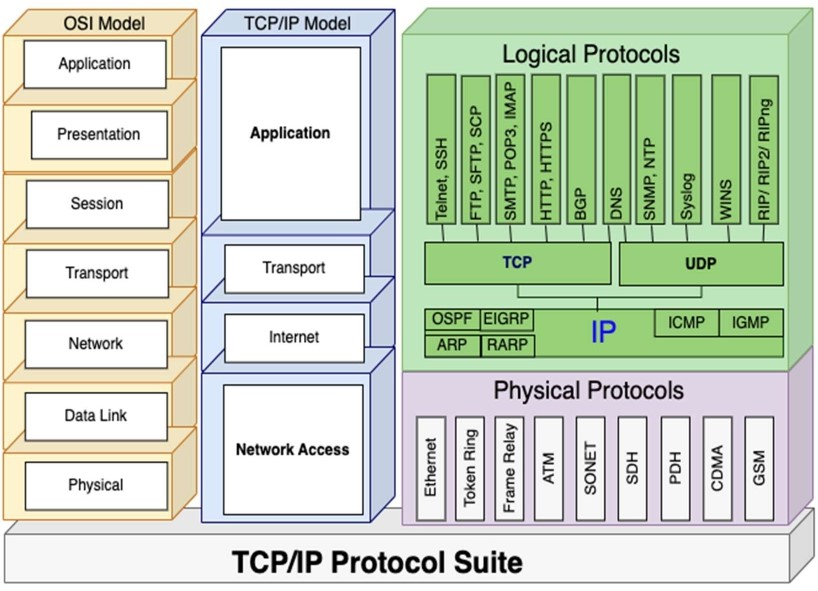
\includegraphics[width=0.8\textwidth]{diagram.jpg}
            \caption{TCP/IP Model}
        \end{figure}
        You job is to   

        \begin{solution}
            \begin{parts}
                \part
                \textbf{Application Layer:} FTP (File Transfer Protocol) is a protocol used for transferring files between devices over a network. It provides a standard way to upload and download files, manage directories, and authenticate users.
                \part
                \textbf{Transport Layer:} TCP (Transmission Control Protocol) is a connection-oriented protocol that provides reliable, error-checked data delivery between devices. It establishes a connection, manages data transfer, and ensures data integrity by retransmitting lost packets and acknowledging received packets.
                \part
                \textbf{Internet Layer:} ICMP (Internet Control Message Protocol) is a protocol used to send error messages and control messages between devices on an IP network. It is used to diagnose network problems, report errors, and manage network traffic.
                \part
                \textbf{Network Access Layer:} GSM (Global System for Mobile Communications) is a standard used in cellular networks to provide voice and data services to mobile devices. It defines the radio interface, network architecture, and signaling protocols used in mobile communication.
            \end{parts}
            \begin{thebibliography}{9}
                \bibitem{author1}
                \url{https://www.geeksforgeeks.org/tcp-ip-model/}
                
                \bibitem{author2}
                \url{https://bcalabs.org/subject/tcp-ip-model}
            \end{thebibliography}
        \end{solution}

        \question[5 $\times$ 1 = 10]
        Internet access is normally provided in different parts of the world through a number of International ISPs (Internet Service Providers), Regional ISPs, and National ISPs.
        \begin{parts}
            \part{Your task is to find out the most popular ISP in each of the above category.}
            \part{Find out the Flagship product/service offered by each of the ISP for highspeed Internet access.}
        \end{parts}

        \begin{solution}
            \begin{parts}
                \part
                \textbf{International ISP:} Comcast Xfinity: Comcast Xfinity is one of the largest ISPs in the world, providing internet services in multiple countries.\\
                \textbf{Regional ISP:} Spectrum: Spectrum is a leading regional ISP in the United States, offering internet services in multiple states.\\
                \textbf{National ISP:} AT\&T: AT\&T is a national ISP in the United States, providing internet services across the country.
                \part
                \textbf{Comcast Xfinity:} Xfinity Gigabit Internet: This service offers speeds up to 1,200 Mbps, making it ideal for heavy internet users, gamers, and households with multiple devices.
                \textbf{Spectrum:} Spectrum Internet Ultra: This service offers speeds up to 400 Mbps, making it ideal for streaming, gaming, and downloading large files.
                \textbf{AT\&T:} AT\&T Fiber: This service offers speeds up to 1,000 Mbps, making it ideal for households with multiple devices and heavy internet users.
            \end{parts}
            \begin{thebibliography}{9}
                \bibitem{author1}
                \url{https://www.xfinity.com/gig}
                
                \bibitem{author2}
                \url{https://www.reviews.org/internet-service/best-internet-service-providers/}
            \end{thebibliography}
        \end{solution}
    \end{questions}
\end{document}
